\lecture{25}{December 1, 2025}{Introduction to Compressible Flow}

\section{Introduction to Compressible Flow}
Any flow in which density variation is not negligible is termed \textit{compressible}.
In general fluids are never compressible and gasses are compressible, when the Mach number $M \equiv V / c > \num{0,3}$ where $c$ is the local speed of sound and $V$ is the velocity.
Flows with speed less than the speed of sound $M < 1$ are called subsonic.
Flows with speeds greater than the speed of sound are \textit{supersonic}.
Flows with $\num{0,9} < M < \num{1,2}$ are talled \textit{transonic} and flows with $5<M$ are called \textit{hypersonic}.

\subsection{Propagation of Sound Waves}

\subsubsection{Speed of Sound}
The speed of sound $c$ is an important property in compressible fluid flow.
The Mach number $M$ is defined as
\begin{equation*}
  M \equiv \frac{V}{c}
\end{equation*}
where $V$ is the speed of the fluid.

We consider the propagation of a sound wave of infinitesimal strength into an undisturbed medium, shown on \Cref{fig:f12_1a}.
We want to relate the speed of wave propagation $c$ to fluid property changes across the wave.
We denote the pressure and density in the undisturbed medium by $p$ and $\rho$ respectively.
Passage of the wave will cause these to undergo infinitesimal changes to become $p + \mathrm{d}p$ and $\rho + \mathrm{d}\rho$. 
Since the wave propagates into a stationary fluid, the velocity ahead of the wave $V_x$ is zero.
The magnitude of the velocity behind the wave $V_x + \mathrm{d}V_x$ will thus simply be $\mathrm{d}V_x$.

The flow of \Cref{fig:f12_1a} appears unsteady to a stationary observer, viewing the wave motion from a fixed point.
However, the flow appears steady to an observer located \textit{on} an inertial control volume moving with a segment of the wave as shown on \Cref{fig:f12_1b}.
The velocity approaching the control volume is then $c$ and the velocity leaving is $c - \mathrm{d}V_x$.

\begin{figure} [ht]
  \begin{subfigure}{0.46\linewidth}
    \centering
    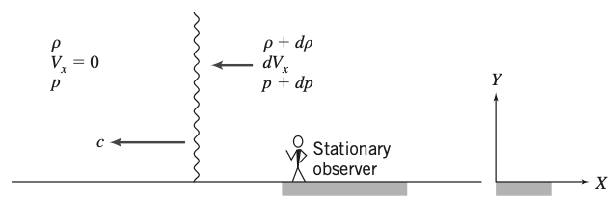
\includegraphics[width=\linewidth]{./figures/f12_1a.png}
    \caption{Propagating wave}
    \label{fig:f12_1a}
  \end{subfigure}
  \begin{subfigure}{0.46\linewidth}
    \centering
    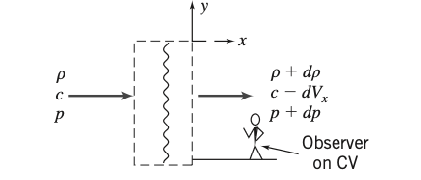
\includegraphics[width=\linewidth]{./figures/f12_1b.png}
    \caption{Inertial control volume moving with wave, velocity $c$}
    \label{fig:f12_1b}
  \end{subfigure}
  \caption{Propagating sound wave showing control volume chosen for analysis.}
\end{figure}

Assuming steady flow and uniform flow at each section the continuity equation is
\begin{equation*}
  \int_{\mathrm{CS}} \rho \Vec{V} \cdot \mathrm{d}\Vec{A} = 0
.\end{equation*}
which can also be written as
\begin{equation*}
  \mathrm{d}V_x = \frac{c}{\rho} \mathrm{d}\rho
.\end{equation*}

Furthermore, assuming negligible body forces the momentum equation becomes:
\begin{equation*}
  F_{S_x} = \int_{\mathrm{CS}} V_x \rho \Vec{V} \cdot \mathrm{d}\Vec{A}
.\end{equation*}

The only surface acting in the $x$ direction on the control volume of \Cref{fig:f12_1b} are due to pressure.
The upper and lower areas have zero friction as the areas are infinitesimal.
This leaves us with:
\begin{equation*}
  \mathrm{d}V_{x} = \frac{1}{\rho c} \mathrm{d}p
.\end{equation*}
Combining this with the previous expression for $\mathrm{d}V_x$, we obtain
\begin{equation*}
  \mathrm{d}V_x = \frac{c}{\rho} \mathrm{d}\rho = \frac{1}{\rho c} \mathrm{d}p
\end{equation*}
from which
\begin{equation*}
  \mathrm{d}p = c^2 \mathrm{d}\rho
\end{equation*}
or
\begin{equation*}
  c^2 = \frac{\mathrm{d}p}{\mathrm{d}\rho}
.\end{equation*}
This indicates that the speed of sound depend on how the pressure and density of the medium are related.
Sound waves are infinitesimal and happen quickly, hence they propagate isentropically.
Therefore, if we express $p$ as a function of density and entropy $p = p(\rho,s)$, then
\begin{equation*}
  \mathrm{d}p = \left( \frac{\partial p}{\partial s}\right)_s \,  \mathrm{d}\rho + \left( \frac{\partial p}{\partial s}  \right)_{\rho} \, \mathrm{d}s = \left( \frac{\partial p}{\partial \rho} \right)_s \, \mathrm{d}\rho
.\end{equation*}
Therefore:
\begin{equation*}
  c^2 = \frac{\mathrm{d}p}{\mathrm{d}\rho} =  \frac{\partial p}{\partial \rho}  \bigg)_s
\end{equation*}
and
\begin{equation} \label{eq:sos}
  c = \sqrt{\frac{\partial p}{\partial \rho} \bigg)_s}
.\end{equation}

We will now apply \Cref{eq:sos} to solids, liquids, and gases.
For solids and liquids data are usually available on the bulk modulus $E_{\nu}$, which is a measure of how a pressure change affects a relative density change:
\begin{equation*}
  E_{\nu} = \frac{\mathrm{d}p}{\frac{\mathrm{d}\rho}{\rho}} = \rho \, \frac{\mathrm{d}p}{\mathrm{d}\rho}
.\end{equation*}
For these media
\begin{equation}
  c = \sqrt{\frac{e_{\nu}}{\rho}}
.\end{equation}

For an ideal gas, the pressure and density in isentropic flow are related as
\begin{equation*}
  \frac{p}{\rho^{k}} = \text{constant}
.\end{equation*}
I.e.:
\begin{align*}
  \frac{\mathrm{d}p}{p}- k \frac{\mathrm{d}\rho}{\rho} &= 0 \\
  \frac{\partial p}{\partial \rho} \bigg)_s = k \frac{p}{\rho}
.\end{align*}
But $p / \rho = RT$, so
\begin{equation}
  c = \sqrt{kRT}
\end{equation}
for an ideal gas.

\subsubsection{Supersonic Motion -- The Mach Cone}
We consider a point source of sound that emits a pusle every $\Delta t$ seconds.
Each pulse expands outwards from its origination point at the speed of sound $c$, so at any instant $t$ the pulse will be a sphere of radius $ct$ centered at the pulse's origination point.
We want to investigate what happens if the point source itself is moving.
There are four possibilities, each shown on \Cref{fig:f12_2}.

\begin{figure} [ht]
  \centering
  \begin{subfigure}{0.45\linewidth}
    \centering
    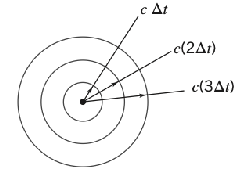
\includegraphics[width=0.8\linewidth]{./figures/f12_2a.png}
    \caption{$V = 0$: Stationary source}
    \label{fig:f12_2a}
  \end{subfigure}
  \begin{subfigure}{0.45\linewidth}
    \centering
    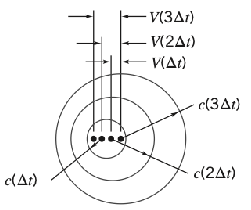
\includegraphics[width=0.8\linewidth]{./figures/f12_2b.png}
    \caption{$V < c$: Doppler shift}
    \label{fig:f12_2b}
  \end{subfigure}
  \\
  \begin{subfigure}{0.45\linewidth}
    \centering
    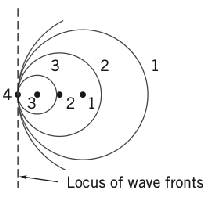
\includegraphics[width=0.8\linewidth]{./figures/f12_2c.png}
    \caption{$V = c$}
    \label{fig:f12_2c}
  \end{subfigure}
  \begin{subfigure}{0.45\linewidth}
    \centering
    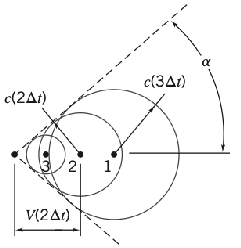
\includegraphics[width=0.8\linewidth]{./figures/f12_2d.png}
    \caption{$V > c$: Supersonic motion}
    \label{fig:f12_2d}
  \end{subfigure}
  \\
  \begin{subfigure}{0.8\linewidth}
    \centering
    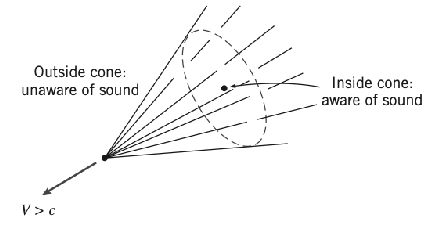
\includegraphics[width=0.6\linewidth]{./figures/f12_2e.png}
    \caption{$M > 1$: The Mach cone}
    \label{fig:f12_2e}
  \end{subfigure}
  \caption{Propagation of sound waves from a moving source: The Mach cone.}
  \label{fig:f12_2}
\end{figure}

\begin{enumerate}
  \item $V = 0$.
    The point is \textit{stationary}.
    \Cref{fig:f12_2a} shows the conditions for the scenario after $3 \Delta t$ seconds.
    The first pulse has expanded to a sphere of radius $c (3 \Delta t)$, the second to a sphere of radius $c (2 \Delta t)$, and the third to a sphere of radius $c(\Delta t)$; a new pulse is about to be emitted.
    The pulses therefore constitute a set of ever-expanding concentric spheres.
  \item $0 < V < c$.
    The point source moves to the left at \textit{subsonic} speed.
    \Cref{fig:f12_2b} shows the conditions for the scenario after $3 \Delta t$ seconds.
    The source is shown at times $t = 0, \Delta t, 2 \Delta t$, and $3 \Delta t$.
    The first pulse har expanded to a sphere radius $c (3 \Delta t)$ centered where the source was originally, the second to a sphere of radius $c(2\Delta t)$ centered where the source was at time $t$ and so on.
    Again, the pulses constitute a set of ever-expanding spheres, except now they are not concentric.
    The pulses are all propagating at constant speed $c$.
    Note that an observer ahead of the source will hear the pulses at a higher frequency than an observer behind the source.
    This is known as the Doppler effect.
    Also, note that an observer ahead of the sound will hear the source \textit{before} the source itself reaches the observer.
  \item $V = c$.
    The point source moves to the left at \textit{sonic} speed.
    \Cref{fig:f12_2c} shows conditions after $3\Delta t$ seconds.
    The source is shown at times $t = 0$, $\Delta t$, $2 \Delta t$, and $3 \Delta t$.
    The first pulse has expanded to sphere 1 of radius $c (3\Delta t)$ centered at point 1, the second to sphere 2 of radius $c(2\Delta t)$ centered at point 2 and so on.
    We can see once more that the pulses constitute a set of ever-expanding spheres, except now they are tangent to one another on the left.
    The pulses are all expanding at constant speed $c$, but the source is moving at speed $c$, with the result that the source and all its pulses are travelling together to the left.
    Here we note that an observer who is ahead of the source will \textit{not} hear the pulses before the source reaches the observer.
    Secondly, over time an unlimited number of pulses will accumulate at the front of the source lading to a sound wave of unlimited amplitude.
  \item $V>c$.
    The point source moves to the left at \textit{supersonic} speed.
    \Cref{fig:f12_2d} shows the conditions after $3 \Delta t$ seconds.
    We can see once more that the pulses constitute a set of ever-expanding spheres, except now the source is moving so fast it moves ahead of each sphere that it generates.
    For supersonic motion, the spheres generate what is called a \textit{Mach cone} tangent to each sphere.
    In this case, an observer who is ahead of the source will not hear the pulses until after the source passes the observer.
    The region inside the cone is called the \textit{zone of action} and that outside the cone the \textit{zone of silence} as shown in \Cref{fig:f12_2e}.
    From geometry, we see from \Cref{fig:f12_2d}, that
    \begin{equation*}
      \sin \alpha = \frac{c}{V} = \frac{1}{M}
    .\end{equation*}
    or
    \begin{equation}
      \alpha = \sin^{-1} \frac{1}{M}
    .\end{equation}
\end{enumerate}

\subsection{Reference State: Local Isentropic Stagnation Properties}
In our study of compressible flow, we will discover that, in general, \textit{all} properties $(p, T, \rho, u, s, V)$ may be changing as the flow proceeds.
We need to obtain reference conditions that we can use to relate conditions in a flow from point to point.
For any flow, a reference condition is obtained when the fluid is brought to rest either in reality or conceptually.
We will call this the \textit{stagnation condition}, and the property values $(p_0, T_0, \rho_0, u_0, h_0, s_0)$ at this state the \textit{stagnation properties}.
The stagnation state is defined by an isentropic process, in which there will is no friction, no heat transfer, and no ``violent'' events.
Hence, the properties we obtain will be the \textit{local isentropic stagnation properties} and, each point in the flow will have its own, or local, isentropic stagnation properties.
This is depicted on \Cref{fig:f12_4} showing a flow from state 1 to some new state 2.
The local isentropic stagnation properties for each state is obtained by isentropically bringing the fluid to rest, are also shown.
Hence, $s_{0_1} = s_1$ and $s_{0_2} = s_2$.
If the flow is isentropic, $s_1 = s_2 = s_{0_1} = s_{0_2}$, so the stagnation states are identical; if it is \textit{not} isentropic, then $s_{0_1} = s_{0_2}$.

\begin{figure} [ht]
  \centering
  
\includegraphics[width=0.8\linewidth]{./figures/f12_4.png}
  \caption{Local isentropic stagnation properties}
  \label{fig:f12_4}
\end{figure}

We recall the Bernoulli equation
\begin{equation*}
  \frac{p}{\rho} + \frac{V^2}{2} + gz = \text{constant}
\end{equation*}
valid for a steady, incompressible, frictionless flow along a streamline.
This is valid for an incompressible isentropic process because it is reversible (frictionless and steady) and adiabatic.
It was previously shown that the Bernoulli equation leads to
\begin{equation*}
  p_0 = p + \frac{1}{2}\rho V^2
.\end{equation*}
The gravity term drops out because we assume the reference state is at the same elevation as the actual state, and in any event in external flows it is usually much smaller than the other terms.

\subsubsection{Local Isentropic Stagnation Propertied for the Flow of an Ideal Gas}
For a compressible flow we can derive the isentropic stagnation relations by applying the mass conservation and momentum equations to a differential control volume, and then integrating.
For the process shown schematically on \Cref{fig:f12_4}, we can depict the process from state 1 to the corresponding stagnation state by imagining the control volume shown in \Cref{fig:f12_5}.

\begin{figure} [ht]
  \centering
  
\includegraphics[width=0.8\linewidth]{./figures/f12_5.png}
  \caption{Compressible flow in an infinitesimal stream tube.}
  \label{fig:f12_5}
\end{figure}

For steady flow and uniform flow at each section the continuity equation reduces to:
\begin{align} \label{eq:coneq}
  \int_{\mathrm{CS}}\rho \Vec{V} \cdot \mathrm{d}\Vec{A} &= 0 \nonumber \\
  \left( - \rho V_x A \right) + \left( \left( \rho + \mathrm{d}\rho \right)\left( V_x + \mathrm{d}V_x \right)\left( A + \mathrm{d}A \right) \right) &= 0 \nonumber \\
  \left( \rho + \mathrm{d}\rho \right)\left( V_x + \mathrm{d}V_x \right)\left( A + \mathrm{d}A \right) &= \rho V_x A
.\end{align}
For negligible body forces and frictionless flow the momentum equation reduces to
\begin{equation*}
  F_{S_x} = \int_{\mathrm{CS}}V_x \rho \Vec{V} \cdot \mathrm{d}\Vec{A}
.\end{equation*}
The surface forces acting on the infinitesimal control volume are
\begin{equation*}
  F_{S_x} = \mathrm{d}R_x + p A - \left( p + \mathrm{d}p \right)\left( A + \mathrm{d}A \right)
.\end{equation*}
The force $\mathrm{d}R_x$ is applied along the stream boundary as shown in \Cref{fig:f12_5}, where the average pressure is $p + \mathrm{d}p / 2$, and the area component in the $x$ direction is $\mathrm{d}A$.
There is no friction, thus,
\begin{equation*}
  F_{S_x} = \left( p + \frac{\mathrm{d}p}{2} \right)\mathrm{d}A + p A - \left( p + \mathrm{d}p \right) \left( A + \mathrm{d}A \right)
\end{equation*}
or
\begin{equation*}
  F_{S_x} = - \mathrm{d}p A
.\end{equation*}
Substituting this result into the momentum equation gives
\begin{equation*}
  - \mathrm{d}p A = V_x \left( - \rho V_x A \right) + \left( V_x + \mathrm{d}V_x \right) \left(  \left( \rho + \mathrm{d}\rho \right) \left( V_x + \mathrm{d}V_x \right) \left( A + \mathrm{d}A \right) \right)
\end{equation*}
which may be simplified using \Cref{eq:coneq} to yield
\begin{equation*}
  - \mathrm{d}p A = \left( - V_x + V_x + \mathrm{d}V_x \right) \left( \rho V_x A \right)
.\end{equation*}
Finally,
\begin{equation*}
  \mathrm{d}p = - \rho V_x \, \mathrm{d}V_x = - \rho \, \mathrm{d} \left( \frac{V_x^2}{2} \right)
\end{equation*}
or
\begin{equation*}
  \frac{\mathrm{d}p}{\rho} + \mathrm{d}\left( \frac{V_x^2}{2} \right) = 0
.\end{equation*}
This is a relation among properties during the deceleration process.
In developing this relation, we have specified a frictionless deceleration process.
Before we can integrate between the initial state and final stagnation state, we must specify the relation that exists between pressure $p$ and density $\rho$ along the process path.

Since the deceleration process is isentropic, then $p$ and $\rho$ for an ideal gas are related by the expression
\begin{equation*}
  \frac{p}{\rho^{k}} = \text{constant}
.\end{equation*}

From $p / \rho^{k} = \text{constant} = C$, we get
\begin{equation*}
  p = C \rho^{k} \qquad \text{and} \qquad \rho = p^{\frac{1}{k}} C^{-\frac{1}{k}}
.\end{equation*}
Therefore:
\begin{equation*}
  - \mathrm{d} \left( \frac{V^2}{2} \right) = \frac{\mathrm{d}p}{\rho} = p^{- \frac{1}{k}} C^{\frac{1}{k}} \, \mathrm{d}p
.\end{equation*}
We integrate this equation between the initial state and the corresponding stagnation state
\begin{equation*}
  - \int_{V}^{0} \mathrm{d} \left( \frac{V^2}{2} \right) = C^{\frac{1}{k}} \int_{p}^{p_0} p^{- \frac{1}{k}} \, \mathrm{d}p
\end{equation*}
to obtain
\begin{equation*}
  \frac{V^2}{2} = C^{\frac{1}{k}} \frac{k}{k-1} p ^{\frac{k-1}{k}} \left( \left( \frac{p_0}{p} \right)^{\frac{k-1}{k}}-1 \right)
.\end{equation*}
Since $C^{1 / k} = p^{1 / k} / \rho$,
\begin{equation*}
  \frac{V^2}{2} = \frac{k}{k-1} \frac{p}{\rho} \left( \left( \frac{p_0}{p} \right)^{\frac{k-1}{k}}-1 \right)
.\end{equation*}

As we seek an expression for stagnation pressure, we rewrite as:
\begin{equation*}
  \left( \frac{p_0}{p} \right)^{\frac{k-1}{k}} = 1 + \frac{k-1}{k} \frac{\rho}{p}\frac{V^2}{2}
\end{equation*}
and
\begin{equation*}
  \frac{p_0}{p} = \left( 1 + \frac{k - 1}{k} \frac{\rho V^2}{2p} \right)^{\frac{k}{k-1}}
.\end{equation*}

For an ideal gas, $p= \rho RT$, and hence
\begin{equation*}
  \frac{p_0}{p} = \left( 1 + \frac{k-1}{2} \frac{V^2}{kRT} \right)^{\frac{k}{k-1}}
.\end{equation*}
Also, for an ideal gas, $p = \rho RT$, and hence
\begin{equation*}
  \frac{p_0}{p} = \left( 1 + \frac{k-1}{2} \frac{V^2}{kRT} \right)^{\frac{k}{k-1}}
.\end{equation*}
Also, for an ideal gas the sonic speed is $c = \sqrt{kRT}$, and thus
\begin{align*}
  \frac{p_0}{p} &= \left( 1 + \frac{k-1}{2} \frac{V^2}{c^2} \right)^{\frac{k}{k-1}} \\
  \frac{p_0}{p} &= \left( 1 + \frac{k-1}{2} M^2 \right)^{\frac{k}{k-1}}
.\end{align*}
This equation enables us to calculate the local isentropic stagnation pressure at any point in a flow field of an ideal gas, provided we know the static pressure and Mach number at that point.

Hence, the equations for determining the local isentropic stagnation properties of an ideal gas are
\begin{align}
  \frac{p_0}{p} &= \left( 1 + \frac{k-1}{2}M^2 \right)^{\frac{k}{k-1}} \\
  \frac{T_0}{T} &= 1 + \frac{k-1}{2}M^2 \\
  \frac{\rho_0}{\rho} &= \left( 1 + \frac{k-1}{2}M^2 \right)^{\frac{1}{k-1}}
.\end{align}


\subsection{Reference State: Critical Conditions}
Stagnation conditions are useful as reference conditions for thermodynamic properties.
A useful reference value for velocity is the \textit{critical speed}, which is the speed $V$ we attain when a flow is either accelerated or decelerated isenotpisally until $M = 1$.
Even if there is no point in a given flow field there the Mach number is equal to unity, such a hypothetical condition still is useful as a reference condition.

Using asterisks to denote conditions at $M = 1$, then by definition,
\begin{equation*}
  V^{*} \equiv c^{*}
.\end{equation*}

At critical conditions the stagnation equations become
\begin{align}
  \frac{p_0}{p^{*}} &= \left( \frac{k+1}{2} \right)^{\frac{k}{k-1}} \\
  \frac{T_0}{T^{*}} &= \frac{k+1}{2} \\
  \frac{\rho_0}{\rho^{*}} &= \left( \frac{k+1}{2} \right)^{\frac{1}{k-1}}
.\end{align}

The critical speed may be written in terms of either critical temperature $T^{*}$ or isentropic stagnation temperature $T_0$.

For an ideal gas $c^{*} = \sqrt{kRT^{*}}$, and thus $V^{*} = \sqrt{kRT^{*}}$.
Since:
\begin{equation*}
  T^{*} = \frac{2}{k+1}T_0
\end{equation*}
we have
\begin{equation*}
  V^{*} = c^{*} = \sqrt{\frac{2k}{k+1} RT_0}
.\end{equation*}


\subsection{Isentropic Flow of an Ideal Gas: Area Variation}
In the absence of heat transfer, friction, and shocks a flow will be reversible and adiabatic.
A general result is
\begin{equation*}
  \dot{m} (s_2 - s_1 ) = \int_{\mathrm{CS}} \frac{1}{T} \left( \frac{\dot{Q}}{A} \right) \, \mathrm{d}A = 0
\end{equation*}
or
\begin{equation*}
  \Delta s = s_2 - s_1 = 0
\end{equation*}
so such a flow is \textit{isentropic}.

We also have that
\begin{equation*}
  T_1 p_1^{\frac{1-k}{k}} = T_2 p_2^{\frac{1-k}{k}} = Tp^{\frac{1-k}{k}} = \text{constant}
\end{equation*}
or its equivalent
\begin{equation*}
  \frac{p_1}{\rho_1^{k}} = \frac{p_2}{\rho_2^{k}} = \frac{p}{\rho^{k}} = \text{constant}
.\end{equation*}
This leads to the set of equations:
\begin{gather} \label{eq:1225}
  \rho_1 V_1 A_1 = \rho_2 V_2 A_2 = \rho V A = \dot{m} = \text{constant} \\
  R_x + p_1 A_1 - p_2 A_2 = \dot{m} V_2 - \dot{m} V_1 \\
  h_{0_1} = h_1 + \frac{V_1^2}{2} = h_2 + \frac{V_2^2}{2} = h_{0_2} = h_0 \\
  s_2 = s_1 = s \\
  p = \rho RT \\
  \Delta h = h_2 - h_1 = c_p \Delta t = c_p \left( T_2 - T_1 \right) \\
  \frac{p_1}{\rho_1^{k}} = \frac{p_2}{\rho^{k}_2} = \frac{p}{\rho^{k}} = \text{constant}
.\end{gather}

\Cref{eq:1225} could be used to analyze isentropic flow in a channel of varying area.
For example if we know the conditions at section 1 we could use these equations to find conditions at some new section 2, where the area is $A_2$.

\subsubsection{Reference Stagnation and Critical Conditions for Isentropic Flow of an Ideal Gas}
Using \Cref{eq:1225} to analyze one-dimensional isentropic flow of an ideal gas, would be somewhat tedious.
Instead, as the flow is \textit{isentropic}, we can find the result in a simpler way
Instead of using \Cref{eq:1225} to compute, e.g. the properties at state 2 from those at state 1, we can use state 1 to determine two reference states, and then use these to obtain properties at state 2.
We need two reference states because the reference stagnation state does not provide area information.

We previously found
\begin{align}
  \frac{p_0}{p} &= \left( 1+ \frac{k-1}{2} M^2 \right)^{\frac{k}{k-1}} \\
  \frac{T_0}{T} &= 1 + \frac{k-1}{2}M^2 \\
  \frac{\rho_0}{\rho} &= \left( 1 + \frac{k-1}{2}M^2 \right)^{\frac{1}{k-1}}
.\end{align}
We note that the \textit{stagnation conditions} are \textit{constant throughout the isentropic flow}.
The critical conditions $M = 1$ are related to the stagnation conditions previously introduced:
\begin{align}
  \frac{p_0}{p^{*}} &= \left( \frac{k+1}{2} \right)^{\frac{k}{k-1}} \\
  \frac{T_0}{T^{*}} &= \frac{k+1}{2} \\
  \frac{\rho_0}{\rho} &= \left( \frac{k+1}{2} \right)^{\frac{1}{k-1}} \\
  V^{*} = c^{*} &= \sqrt{\frac{2k}{k+1}} RT_0
.\end{align}

Although a particular flow may never attain sonic conditions, we still find the critical conditions useful as a reference state.

We can obtain a relation between areas $A$ and $A^{*}$ from the continuity equations and get:
\begin{align} \label{eq:aastarrel}
  \frac{p_0}{p} &= \left( 1 + \frac{k-1}{2}M^2 \right)^{\frac{k}{k-1}} \\
  \frac{T_0}{T} &= 1 + \frac{k-1}{2}M^2 \\
  \frac{\rho_0}{\rho} &= \left( 1 + \frac{k-1}{2}M^2 \right)^{\frac{1}{k-1}} \\
  \frac{A}{A^{*}} &= \frac{1}{M} \left( \frac{1 + \frac{k-1}{2} M^2}{\frac{k+1}{2}} \right)^{\frac{k+1}{2 \left( k-1 \right)}}
.\end{align}
\Cref{eq:aastarrel} provide property relations in terms of the local Mach number, the stagnation conditions, and critical conditions.
